\documentclass{report}

\usepackage{a4}
\usepackage[hypertex]{hyperref}
\usepackage{graphicx}

\begin{document}

\title{Exploring Machine Learning:\\
  The ID3 algorithm}

\author{Mohammed Ibrahim\\
 Computer Science Department\\
  College of Science, Swansea University\\
  Swansea, SA2 8PP, UK
}

\maketitle

\tableofcontents

\chapter{File Format}
\label{sec:fileformat}

\section{File Format}
\label{sec:file}

A file format is a specific way that information is encoded for storage in a computer file. There are different kinds of file formats for different kinds of information. Some file formats are designed for very particular sorts of data.
We are using CSV file to input a data into our application.

\section{Comma-separated values}
\label{sec:csv}

To refer from \cite{Wikipedia_CommaSeparatedValues}(page 1): A comma-separated values(CSV) file stores tabular data(numbers and text)in plain text form. Plain text means that the file is a sequence of characters, with no data that has to be interpreted instead, as binary numbers. A CSV file consists of any number of records, separated by line breaks of some kind; each record consists of fields, separated by some other character or string, most commonly a literal TAB or comma. Usually, all records have an identical sequence of fields.


\section{Identifiers}
\label{sec:ide}

According to \cite{Roberts2000CompleteJava2Certification}(Chapter 1, page 6): An identifier is a name used by a programmer to variable, method, package, class, interfaces or label. Keywords and reserved words can't be used as  identifiers. It must begin with a letter, a dollar sign, or an underscore; identifiers are case sensitive. Identifiers are tokens (also called symbols) which name as language entities. Each variable has a name by which it is identified in the program.


\section{Decision Tree}
\begin{figure}[h]
\centering

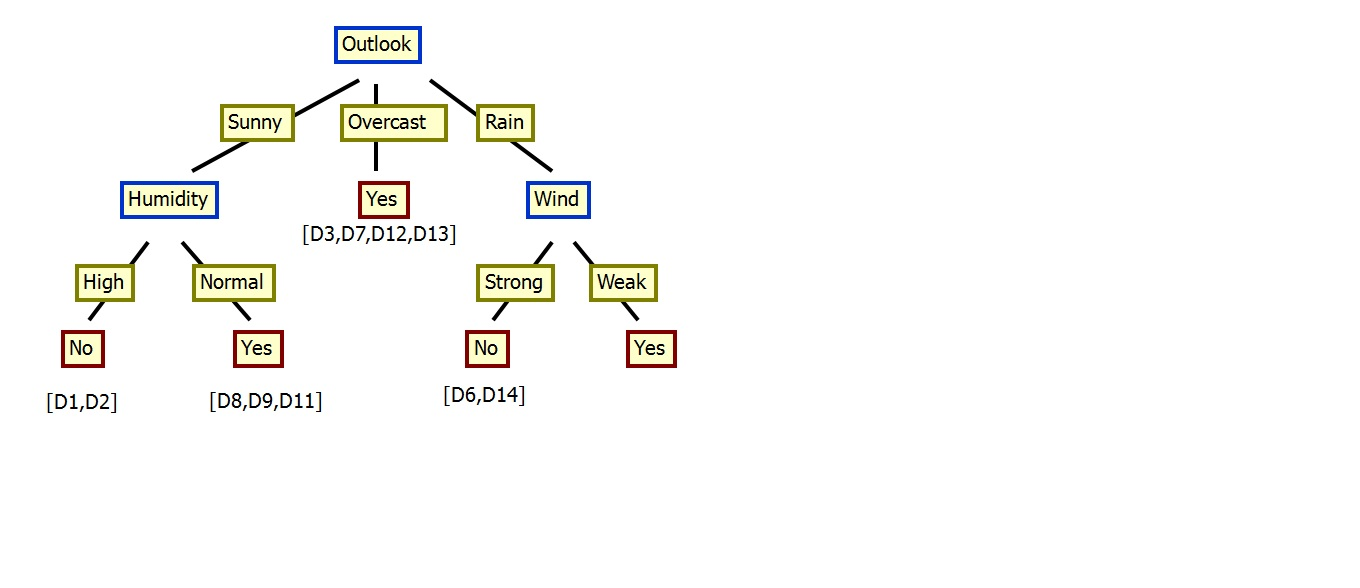
\includegraphics[bb=0 0 1360 588,scale=0.5,keepaspectratio=true]{DecisionTree.jpg}
\caption{Decision Tree}
\end{figure}



\bibliographystyle{plain}
\bibliography{Bibliography}



\end{document}